\section{Logistic Lasso Regression}
\label{sec:p1q2}

An important preprocessing step for Lasso regression (i.e. Logistic regression with the $L_1$-regularization) is the standardization of the features, which has been done in the preprocessing step.

We trained a Lasso regression classifier using a logistic model with SGD training and $L_1$-regularization. The loss function is set to log-loss which is suitable for binary classification.

We optimized for the $\alpha$ parameter (the amount of $L_1$ regularization) using a grid search on 31 logarithmically-spaced values between $0.001$ and $1$, choosing $\alpha\approx 0.025$. The grid search optimized for the F1 score, by cross-validation within the training dataset.

The model achieved the (F1) score of $85.9\%$ on the training dataset and the score of $79.2\%$ on the test dataset.

\begin{figure*}
    \centering
    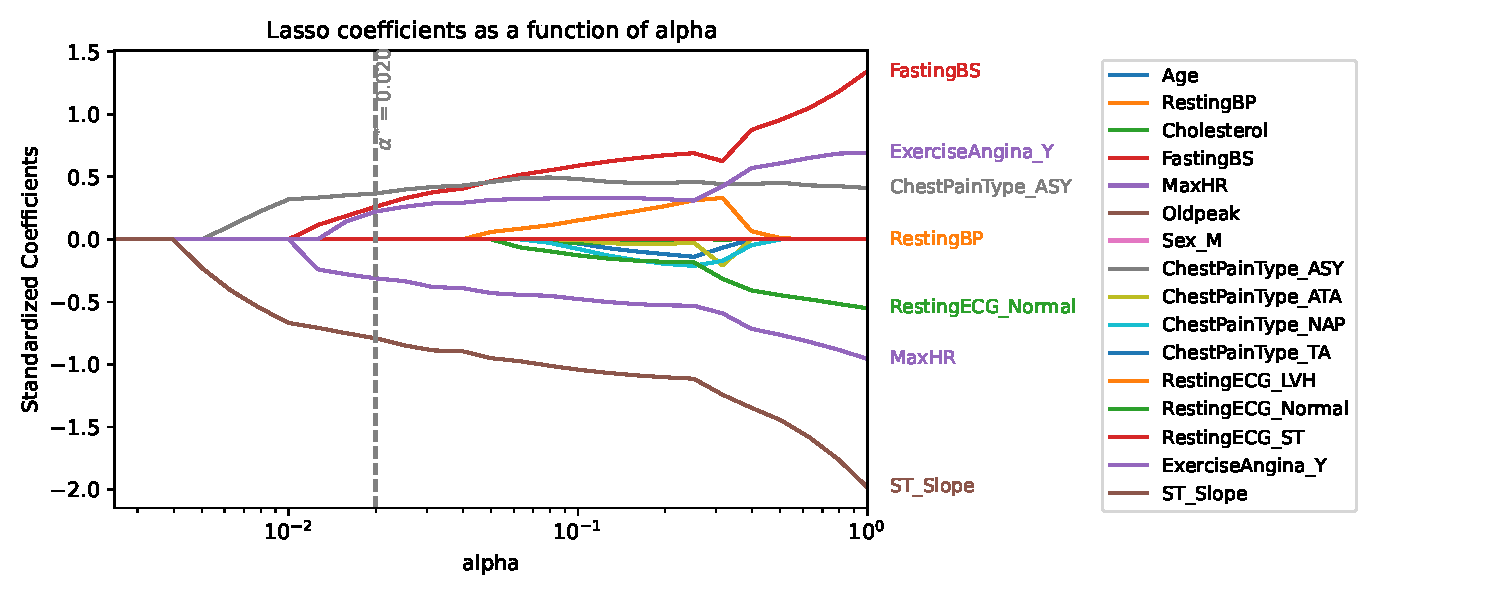
\includegraphics[width=0.9\textwidth]{images/lasso_coef_f.pdf}
    \caption{Lasso coefficients as a function of $\alpha$. The horizontal line corresponds to the highest-scoring $\alpha=0.025$}
    \label{fig:lasso_coef_f}
\end{figure*}

\autoref{fig:lasso_coef_f} shows the importance of each feature for each considered value of $\alpha$. We observe that with decreasing $\alpha$, the model has more features with positive coefficients, as expected.

We also observe that the set of features highly correlated with Heart disease is similar to those marked as most relevant by the Lasso regression, i.e. those with positive coefficients at $\alpha=0.025$. Namely, the features marked as relevant by Lasso regression are: \texttt{ST\_Slope}, \texttt{ChestPainType\_ASY} (a one-hot flag of the \texttt{ChestPainType} feature), \texttt{MaxHR}, \texttt{FastingBS}, and \texttt{ExerciseAngina\_Y}.

Further, we attempted fitting another Lasso regression which would only use those features marked as relevant. For this second regression, a similar grid-search approach found the same $\alpha$ optimal. The second model achieved slightly higher score on the train dataset, but made no difference on the test dataset; see \autoref{tab:lasso_selection}.

\begin{table}
\centering
\begin{tabular}{l|l|l|}
 & Train (F1) & Test (F1) \\ \hline
Lasso-all & $85.9\%$ & $79.2\%$ \\ \hline
Lasso-selected & $86.0\%$ & \textbf{$79.2\%$} \\ \hline
\end{tabular}
\caption{Comparison of the F1 scores of the Lasso regression with all features, and with only the selected 5 features.}
\label{tab:lasso_selection}
\end{table}
